\documentclass[11pt, twocolumn, a4paper]{article}

\usepackage{graphicx}
\usepackage{booktabs}
\usepackage{multirow}
\setlength{\oddsidemargin}{0.0 cm}
\setlength{\evensidemargin}{0.0 cm}
\setlength{\topmargin}{-1cm}
\setlength{\textheight}{24 cm}
\setlength{\textwidth}{16 cm}

\newcommand{\ttbarm}{\mathrm{t \overline{t} \; }}
\newcommand{\ttbar}{$\mathrm{t \overline{t} \; }$}
\newcommand{\ttbars}{${t \overline{t} \; }$}
\newcommand{\ttbarsm}{{t \overline{t} \; }}
\newcommand{\ttW}{{t \overline{t} W }}
\newcommand{\ttZ}{{t \overline{t} Z }}


\pagestyle{plain}

\setlength{\parindent}{0in}

\usepackage[
  locale=DE,
  separate-uncertainty=true,
  decimalsymbol=.,
  per-mode=symbol-or-fraction,
]{siunitx}
\DeclareSIUnit\permille{\text{\textperthousand}}
\usepackage{textcomp}
\usepackage{amsmath,amssymb}
\usepackage{cancel}

\usepackage[verbose]{placeins}

\begin{document}
\thispagestyle{empty}

\author{Salvatore La Cagnina}

\title{Summary of `D0 Collaboration, {\it 'Simultaneous measurement of forward-backward asymmetry and top polarization in dilepton final states from \ttbars production at the Tevatron'}}
\maketitle

%#############################################################################
%###########################Into + Eckdaten###################################
%#############################################################################
The D0 collaboration presents a simultaneous measurement of the forward-backward
asymmetry $A^{\ttbarsm}$ and the top polarization $kP$ at the Tevatron in dilepton final states of \ttbars.
The analyzed events orginate from $p \overline{p}$ collisions and correspond to
an inverse luminosity of $\mathcal{L} = \SI{9.7}{fb^{-1}}$.
Due the center of mass energy of $\sqrt{s}=\SI{1.96}{TeV}$ and the collision of
protons with anti-protons, the production of \ttbars is induced from quark anti-quark
anhilation and not gluon fusion making this measurement possible.\\
%#############################################################################
%#############################Motivation######################################
%#############################################################################
The Standard Model (SM) of particle physics predicts values for the asymmetry and polarization.
These values can also be extracted from Beyond Standard Model models like axigluon models\cite{axi}.
Therefore, this analysis yields a test of those predictions with the experimental results.
In this analysis the theory predictions are calculated for both SM and the axigluon models.\\
%#############################################################################
%###########################Event Topo u Untergr##############################
%#############################################################################
Using the dilepton final state of \ttbars the signature of the events consist
of two jets with high transverse momentum $p_T$ originating from the hadronization
of two b quarks, two high $p_T$ leptons and missing transverse Energy 
$\cancel{E}_T^\text{miss}$ from the undetected neutrinos.
Due to this topology, processes with similar shapes lead to background contributions.
The main processes for background are ${Z \rightarrow ll}$ with ${l=e,\mu,\tau}$,
diboson production $(WW,WZ,ZZ)$ but also $W$+jets and multijet events considering 
misreconstruction from jets as leptons.
The last two background sources are considered "instrumental background" and 
their contribution is derived from data.
Whereas, the firstly mentioned backgrounds are estimated using Monte Carlo (MC) samples.
Furthermore, certain event selection criteria such as isolation criteria ,which 
suppresses misidentification of muons that originate from hadron decays as prompt ones, 
are applied in order to constrain the contribution of background events.\\
%#############################################################################
%##########################Matrixelement Methode##############################
%#############################################################################
In order to yield a result for $A^{\ttbarsm}$ and $kP$, distributions that are related to these
values are extracted from the data using a matrix element method\cite{matrix}.
The searched distributions are $\Delta{y}_{\ttbarsm}$, which represents the difference in rapidity
of the top and anti-top, and $cos(\theta^{\pm})$ where $\theta$ is the angle between the (anti-)lepton and
the (anti-)top.
The matrix element method consists of a few steps.
First, for every event a likelihood distribution is calculated.
Second, the likelihood variables are constrained to a set of 4 to 6 variables depending on the lepton final states.
Third, the likelihood distributions for $\Delta{y}_{\ttbarsm}$ and $cos(\theta^{\pm})$ are extracted by integration of the likelihood.
Lastly, these likelihood distributions are accumulated and used in order to obtain a result for the asymmetry and polarization.
It is noticeable, that $A^{\ttbarsm}$ and $kP$ are not calculated using the maximum likelihood value of the $\Delta{y}_{\ttbarsm}$ and $cos(\theta^{\pm})$ but rather by using the entire likelihood distribution.\\
However, these extracted "raw" values called $A^{\ttbarsm}_\text{raw}$ and $kP_\text{raw}$ do not account for dilution effects of the detector, resolution effects of the reconstruction and the simplified constrains in the matrix element measurement, used in order to minimize the likelihood variables.
Consequently, a calibration of the "raw" values has to be implemented.
Using MC, a calibration matrix $C$, offset vector $O$ and reweight factors for the $\Delta{y}_{\ttbarsm}$ and lepton angular distribution are calculated.
So, the true values for $A^{\ttbarsm}$ and $kP$ can be calculated using
\begin{equation*}
	\binom{A^{\ttbarsm}_\text{raw}}{kP_\text{raw}} = C \cdot \binom{A^{\ttbarsm}}{kP} + O \,.
\end{equation*}
%#############################################################################
%##########################Unsicherheiten#####################################
%#############################################################################
The main contributions to the systematic uncertainty arise from the variable variation of the model and from the hadronisation and showering from the signal modeling. 
However, the main uncertainty of this measurement is found within the statistical uncertainty caused by the lack of analyzed events.
One specific detail about the uncertainties in this analysis is the statistical correlation 
between the measured quantities and the additional systematic uncertainty caused by the calibration of the 
raw values of $A^{\ttbarsm}$ and $kP$.\\
%#############################################################################
%##################################Ergebnisse#################################
%#############################################################################
The results of the calibrated values for the asymmetry and the polarization are
\begin{align*}
	A^{\ttbarsm} &= \SI[parse-numbers=false]{(15.0 \pm 6.4 (stat.) \pm 4.9 (syst.))}{\%}\\
	kP &= \SI[parse-numbers=false]{(7.2 \pm 10.5 (stat.) \pm 4.2 (syst.))}{\%}
\end{align*}
with a correlation of \SI{-56}{\%} between them.
These values are in agreement with the SM value of ${A^{\ttbarsm} = \SI[parse-numbers=false]{(9.5 \pm 0.7)}{\%}}$ and ${kP = \SI[parse-numbers=false]{(-0.19 \pm 0.05)}{\%}}$.
This agreement can be seen in figure \ref{fig:SMV} due to the SM value being located in the \SI{68}{\%} confidence level interval of this measurement.
However, all the considered BSM axigluon theories are also in agreement with the measurement regarding figure \ref{fig:SMV}. 
\begin{figure}
	\centering
	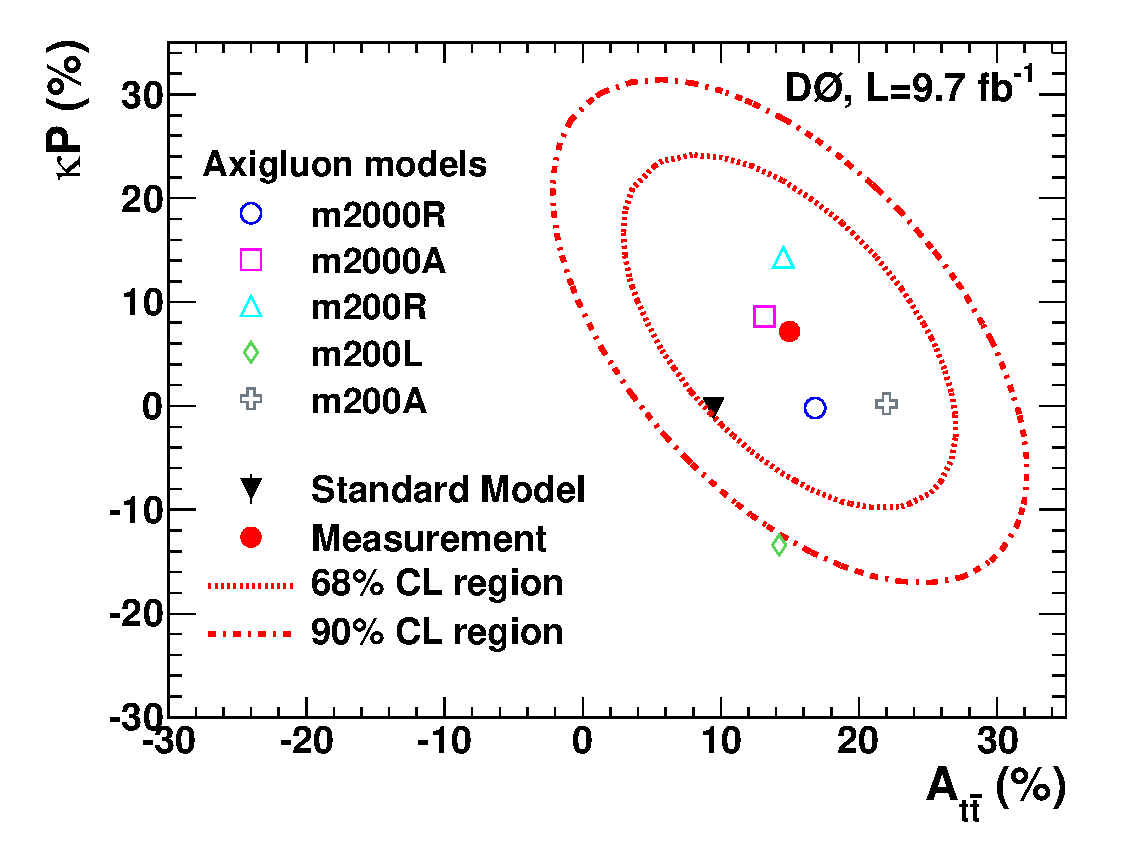
\includegraphics[width=0.5\textwidth]{afb_polar_measurement_statsyst_bsm-eps-converted-to.pdf}
	\caption{Asymmetry and polarization of the SM and other axigluon models compared to the measurement. The \SI{68}{\%} and \SI{90}{\%} confidence level regions of the measurement are shown as dotted lines.\cite{paper}}
	\label{fig:SMV}
\end{figure}
By constraining one of the variables to its SM value, the other value can be recalculated.
This leads to an result of 
\begin{align*}
	A^{\ttbarsm} &= \SI[parse-numbers=false]{(17.5 \pm 6.3)}{\%}\\
	kP &= \SI[parse-numbers=false]{(11.3 \pm 9.3)}{\%}
\end{align*}
with fixed $kP$ and $A^{\ttbarsm}$ values respectively.
Finally, for $A^{\ttbarsm}$ a previous measurement in the lepton+jets channel \cite{olde} can be combined with the measurement value
resulting in an value for the asymmetry of $A^{\ttbarsm}=\SI[parse-numbers=false]{(11.8 \pm 2.8)}{\%}$.\\
%#############################################################################
%##################################Einordnung#################################
%#############################################################################
This measurement yields no statement towards one of the BSM theories and is compatible with the SM prediction.
However, this analysis shows how a measurement of the asymmetry and polarization can be extracted from a $p\overline{p}$
collider experiment.
Unfortunately the LHC cannot contribute towards this, due to the main production channel of \ttbars being gluon fusion where no asymmetry is present.
Consequently, in order to obtain a more convincing result, this analysis should be repeated using more data from Tevatron.
Therefore, lowering the high statistical uncertainty. 

\begin{thebibliography}{99}
\bibitem{paper} D0 Collaboration,
Simultaneous measurement of forward-backward asymmetry and top polarization in dilepton final states from \ttbars production at the Tevatron, Phys. Rev. D 92 (2015) 052007.
\bibitem{axi}O. Antunano, J. H. K\"uhn, and G. Rodrigo, Top quarks, axigluons, and charge asymmetries at hadron colliders, Phys. Rev. D 77 014003 (2008).
\bibitem{matrix}K. Kondo, Dynamical Likelihood Method for Reconstruction of Events with Missing Momentum. I. Method and Toy Models, J. Phys. Soc. Jap. 57 4126 (1988). 
\bibitem{olde}D0 Collaboration, Measurement of the forward-backward asymmetry in top quark-antiquark production in $p\overline{p}$ collisions using the $\mathrm{lepton}\mathbf{+}\mathrm{jets}$ channel, Phys. Rev. D 90 072011 (2014).

\end{thebibliography}



\end{document}












%\begin{figure}[ht!]
%  \begin{center}
%    \includegraphics[width=0.5\textwidth]{plot.pdf}
%    \caption{A figure caption~\cite{brandt}.}
%    \label{fig:fig1}
%  \end{center}
%\end{figure}

% In this paper a measurement of the $t \overline{t} Z$ and $t \overline{t} W$ production cross section is presented.
% The sample contains $\SI{3.2}{fb^{-1}}$ of $pp$ collision data at $\sqrt{s} = \SI{13}{TeV}$.
% The data is collected with the ATLAS detector at the LHC at CERN in the year 2015. 
% In order to extract the cross sections, a maximum-likelihood fit is used at differently selected signal and control regions.\\
% %
% %
% This measurement yields a test of the Standard Model (SM) due to new physics possibly changing the production of massive vector bosons together with \ttbars.
% Furthermore, this measurement offers information about the neutral-current coupling of the top quark which can be compared to theoretical SM predictions.
% This measurement has been previously studied for $7$ and $\SI{8}{TeV}$ \cite{paper_alt1,paper_alt2}, however, this study is performed with a higher center of mass energy leading to the increased cross sections of processes.\\
% %
% %
% For this measurement different decay channels are considered.
% They can be separated in three different categories.
% Those are same-sign muon (SS-$\mu$), trilepton and tetralepton.
% The decay requirements for the channels and their correspondence to $\ttW$ and $\ttZ$ can be seen in Table \ref{tab:intro-channels}.
% \begin{table}[htbp]
% \centering
% \caption{\label{tab:intro-channels} Decay modes with assignment to the $\ttW$ or $\ttZ$ process and corresponding channel.\cite{paper}} 
% \resizebox{0.5\textwidth}{!}{
% \begin{tabular}{cccc}
% \toprule
% Process & \ttbar decay & Boson decay & Channel\\
% \midrule
% \multirow{2}{*}{$\ttW$} 
% &  $(\mu^{\pm}\nu b) (q\bar{q} b) $ & $\mu^{\pm}\nu$ & SS dimuon\\
% & $ (\ell^{\pm}\nu b) (\ell^{\mp}\nu b)$ & $\ell^{\pm}\nu$ & Trilepton\\
% \midrule
% \multirow{2}{*}{$\ttZ$} 
% & $(\ell^{\pm}\nu b) (q\bar{q} b)$ & $ \ell^{+}\ell^{-}$ & Trilepton\\
% & $(\ell^{\pm}\nu b) (\ell^{\mp} \nu b)$ & $ \ell^{+}\ell^{-}$ & Tetralepton\\
% \bottomrule
% \end{tabular}}
% \end{table}
% Each of the analysis channels is divided in multiple signal, control and validation regions.
% For the cross sections the signal and control regions are fitted simultaneously.\\
% %
% %
% The monte carlo samples are created using several generators with fixed top and Higgs masses to $m_t=\SI{172.5}{GeV}$ and $m_H=\SI{125}{GeV}.$
% In order to correctly simulate the events, the main backgrounds have to be implemented.
% These are fake leptons, diboson events ($WZ,ZZ$) and other SM processes creating at least three prompt leptons like $Z$+jets or \ttbars + Higgs processes.\\
% \FloatBarrier
% %
% Requiring leptons to be prompt and therefore being isolated reduces the amount of lepton background from hadron decays and misidentified leptons.
% Other cuts and trigger requirement are also added in order to minimize the amount of background events.
% For the different analysis channels and the different signal and control regions different cuts are applied.\\
% The SS-$\mu$ channel has the highest sensitivity in comparison to other lepton channels due to the electron having a much higher charge misidentification.
% The events are chosen by using cuts on the transverse momentum $p_T$, missing transverse momentum $E_T^{miss}$, the scalar sum of $p_T$ called $H_T$ and the number of $b$-tagged jets. 
% The main background are fake leptons so the validation region is chosen so the background estimate which is extracted using the matrix method \cite{MM} can be approved.\\
% %
% In the trilepton channel there are four signal regions, one control region and two validation regions.
% The signal regions are distinguished by their number of $b$-tagged and light jets, by the presence of a $Z$ candidate and the sign of two same flavor leptons.
% This channel is sensitive to $\ttW$ and $\ttZ$ and its main background source is fake leptons but also other previously mentioned background.
% The requirements of this channel which suppresses most other background are one pair of opposite signed same flavor leptons (OSSF) and the invariant mass of them being near the $Z$ mass.
% This is valid for three of the four signal regions the last one having these requirements vetoed.
% The validation regions are used to confirm the background hypothesis and the control region is used to constrain the $WZ$ background normalization for the fit.\\
% %
% The tetralepton channel is used for $\ttZ$ and requires two pairs of (OSSF) leptons.
% Signal regions are chosen by the flavor of the pairs being identical or not and by the number of $b$-tagged jets leading to four different regions.
% The main background is again caused by fake leptons and is suppressed by applying cuts on $p_T$, $H_T$ and the invariant mass of the opposite signed lepton pairs.
% The control region is used to constrain the $ZZ$ background normalization for the fit analogously to the trilepton channel.\\
% %
% %
% The main systematic uncertainties are caused by the reconstruction of the physics object and fake leptons (for $\ttW$), however, the main uncertainty for this measurement is the static uncertainties caused by the overall acceptance of the processes of $\SI{6}{\permille}$ and $\SI{2}{\permille}$ for $\ttZ$ and $\ttW$ respectively.\\
% %
% %
% By simultaneously fitting the control and signal regions using a binned maximum-likelihood fit with systematic uncertainties as nuisance parameters, the cross sections can be extracted.
% They are measured to be 
% ${\sigma_{\ttZ}=\SI[parse-numbers=false]{0.92 \pm 0.29 (stat.) \pm 0.10 (syst.)}{pb}}$ and 
% ${\sigma_{\ttW}=\SI[parse-numbers=false]{1.50 \pm 0.72 (stat.) \pm 0.33 (syst.)}{pb}}$.
% These are consistent with the SM predictions which are calculated in NLO perturbative QCD to be
% ${\sigma_{\ttZ}=\SI[parse-numbers=false]{0.84 \pm 0.09}{pb}}$ and
% ${\sigma_{\ttW}=\SI[parse-numbers=false]{0.60 \pm 0.08}{pb}}$.
% This can also be seen in fig. \ref{fig:theo} since the SM prediction is contained in the $\SI{68}{\%}$ confidence level interval.
% Relying on this measurement, the significance over the background only hypothesis for $\ttW$ is only $\num{2.2}\sigma$ which is not high enough to approve the existence of the $\ttW$ process.
% This is mainly caused because of the high statistical uncertainty, therefore, further analysis with more data have to follow.
% \begin{figure}[h!]
% 	\centering
% 	\includegraphics[width=0.5\textwidth]{paper/ttZ_vs_ttW_2Dfit.pdf}
% 	\caption{Resulting cross section for $\ttW$ and $\ttZ$ compared to the SM prediction. The $\SI{68}{\%}$ and $\SI{95}{\%}$ confidence level for the fit and the one sigma uncertainty for the theory is shown. \cite{paper}}
% 	\label{fig:theo}
% \end{figure}
